\documentclass[conference]{IEEEtran}
\usepackage[T1]{fontenc}
\usepackage[utf8]{inputenc}
\usepackage[spanish,es-noshorthands]{babel}
\usepackage{amsmath,amssymb,graphicx}
\graphicspath{{figuras/}}
\begin{document}
\title{Análisis del movimiento del robot ABB IRB 120\\Hito 2 - Robótica}
\author{\IEEEauthorblockN{Yusep Pantoja, Ramiro Caucota, Alberto Ruiz y Ricardo Velazco}
\IEEEauthorblockA{Ingeniería Mecatrónica\\Universidad Católica Boliviana ``San Pablo'', Tarija, Bolivia\\IMT-342 Robótica}}
\maketitle
\begin{abstract}
En este trabajo conectamos los cálculos necesarios para estudiar el movimiento del robot ABB IRB 120. Partimos de una posición y orientación de la herramienta, calculamos los ángulos de sus articulaciones y comprobamos el resultado. Después generamos una trayectoria LSPB, analizamos una singularidad y estimamos el torque del hombro con un modelo 1R. En el ejemplo estudiado, el movimiento dura 1,288 s y el torque máximo calculado es de 20,55 N\,m. Los resultados se obtuvieron por simulación en Python.
\end{abstract}
\begin{IEEEkeywords}
ABB IRB 120, cinemática inversa, trayectoria LSPB, singularidad, torque.
\end{IEEEkeywords}

\section{Introducción}
El objetivo del Hito 2 es unir los temas de cinemática, trayectorias, Jacobiano y dinámica en un mismo programa \cite{guia}. Para hacerlo, seguimos este orden: definir la pose de la herramienta, encontrar los ángulos del robot, comprobarlos, planificar el movimiento y calcular sus velocidades y torque.

Usamos Python, NumPy y Matplotlib. El trabajo es una simulación del ABB IRB 120 y no incluye pruebas de movimiento con el brazo físico. La pose utilizada es el ejemplo del cuaderno; se puede cambiar para repetir el procedimiento con otras poses.

\section{Modelo del robot}
El IRB 120 tiene seis articulaciones de giro. Usamos los parámetros DH de la Tabla~\ref{tab:dh} para relacionar cada eslabón con el siguiente. Las longitudes están en metros y los cálculos de ángulos se hacen en radianes. En el informe mostramos grados para facilitar la lectura.
\begin{table}[!b]
\caption{Parámetros DH utilizados.}\label{tab:dh}\centering
\begin{tabular}{crrrr}\hline
Eje & $d$ [m] & $a$ [m] & $\alpha$ [$^\circ$] & Ángulo $\theta$\\\hline
1 & 0,290 & 0 & $-90$ & $q_1$\\
2 & 0 & 0,270 & 0 & $q_2-90^\circ$\\
3 & 0 & 0,070 & $-90$ & $q_3$\\
4 & 0,302 & 0 & 90 & $q_4$\\
5 & 0 & 0 & $-90$ & $q_5$\\
6 & 0,072 & 0 & 0 & $q_6+180^\circ$\\\hline
\end{tabular}
\end{table}

El punto de trabajo de la herramienta, llamado TCP, está a 0,150 m de la brida sobre su eje $z$. Para encontrar su pose multiplicamos las seis matrices DH y añadimos esa distancia:
\begin{equation}
T_{TCP}(q)=A_1A_2A_3A_4A_5A_6T_z(0{,}150).
\end{equation}
La distancia del TCP es una elección de nuestro modelo. Al colocar todas las articulaciones en cero, la posición del TCP resulta $(0{,}524;0;0{,}630)$ m.

También tomamos en cuenta los límites de giro y las velocidades de la ficha del fabricante \cite{abb}. Para el ejemplo usamos el 25\% de las velocidades máximas. Como límite de aceleración, suponemos que cada eje puede llegar a esa velocidad en 0,25 s. Este tiempo es un supuesto del programa.

\section{Cinemática inversa y comprobación}
\subsection{Pose de ejemplo}
Partimos de todas las articulaciones en cero. La pose objetivo del TCP es $(0{,}40;0{,}10;0{,}35)$ m, con orientación RPY $(0;180;0)^\circ$. Su matriz es
\begin{equation}
T_d=\begin{bmatrix}
-1&0&0&0{,}40\\
0&1&0&0{,}10\\
0&0&-1&0{,}35\\
0&0&0&1
\end{bmatrix}.
\end{equation}
Esta matriz indica tanto dónde debe estar la herramienta como hacia dónde debe apuntar.

\subsection{Soluciones por el método de Pieper}
Primero encontramos el centro de la muñeca. Para ello, descontamos desde el TCP la extensión de la herramienta y la distancia de la última articulación:
\begin{equation}
p_W=p_{TCP}-(0{,}150+0{,}072)z_6.
\end{equation}
En este caso obtenemos $p_W=(0{,}400;0{,}100;0{,}572)$ m. Después resolvemos los primeros tres ángulos usando la geometría del brazo y la ley de cosenos. Los últimos tres ángulos se calculan con la orientación que falta completar en la muñeca. Usamos \texttt{atan2} para conservar el cuadrante correcto.

El método puede dar hasta ocho soluciones: dos opciones de base, dos de codo y dos de muñeca. Para este objetivo aparecen ocho soluciones geométricas, pero sólo la rama 2 respeta todos los límites articulares. Las otras siete se descartan por superar uno o más límites. Los ángulos elegidos son
\begin{equation}
\begin{split}
q_f[{}^\circ]=[&14{,}036;\ 22{,}667;\ -15{,}700;\\
&0;\ 83{,}034;\ 14{,}036]^T.
\end{split}
\end{equation}

Para comprobarlos, volvemos a calcular la pose mediante cinemática directa y la comparamos con $T_d$. Revisamos posición y orientación, con tolerancias de $10^{-6}$ m y $10^{-6}$ rad. La solución elegida cumple ambas. Esta prueba comprueba las ecuaciones del programa; no mide el error del robot físico.

\section{Trayectoria LSPB}
Una vez definidos los ángulos iniciales y finales, necesitamos decidir cómo cambia cada uno con el tiempo. Usamos LSPB, que divide el movimiento en tres partes: acelerar, mantener velocidad constante y frenar.

Todas las articulaciones comparten el tiempo total $t_f$ y el tiempo de mezcla $t_b$. Para cada eje calculamos la velocidad $V_i$ y la aceleración $a_i$ a partir del cambio de ángulo:
\begin{equation}
V_i=\frac{q_{f,i}-q_{0,i}}{t_f-t_b},\qquad a_i=\frac{V_i}{t_b}.
\end{equation}
En el ejemplo, $t_b=0{,}250$ s y $t_f=1{,}288$ s. El tramo de velocidad constante dura 0,788 s. La articulación 5 es la que fija el tiempo, porque alcanza los límites elegidos de $80^\circ$/s y $320^\circ$/s$^2$. Las demás se ajustan para llegar al mismo tiempo.

\begin{figure}[t]\centering
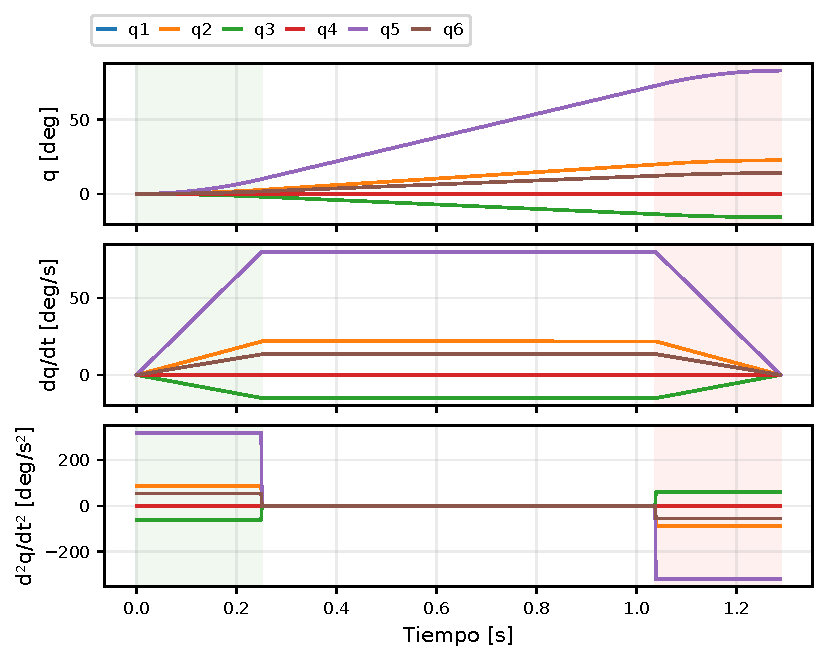
\includegraphics[width=\columnwidth]{C_lspb_perfiles.pdf}
\caption{Posición, velocidad y aceleración de las seis articulaciones.}\label{fig:lspb}
\end{figure}
La Fig.~\ref{fig:lspb} muestra los tres perfiles. El robot parte y termina con velocidad cero. La posición y la velocidad cambian sin saltos; la aceleración cambia por tramos. En este ejemplo, la articulación 4 prácticamente no se mueve.

\section{Jacobiano y singularidad}
El Jacobiano relaciona la velocidad de las articulaciones con la velocidad de la herramienta:
\begin{equation}
\begin{bmatrix}v\\\omega\end{bmatrix}=J(q)\dot q.
\end{equation}
Aquí $v$ es la velocidad lineal y $\omega$ la velocidad angular del TCP. Comprobamos el Jacobiano comparándolo con pequeños cambios de la cinemática directa; el error fue menor que $10^{-8}$.

Para estudiar una singularidad hicimos una prueba separada del movimiento anterior. Fijamos los ángulos $(30;-20;15;40;q_5;60)^\circ$ y acercamos $q_5$ a cero. Cuando llega a cero, los ejes 4 y 6 se alinean y el rango del Jacobiano baja de 6 a 5. Esto significa que la herramienta pierde una dirección de movimiento instantáneo.

\begin{figure}[t]\centering
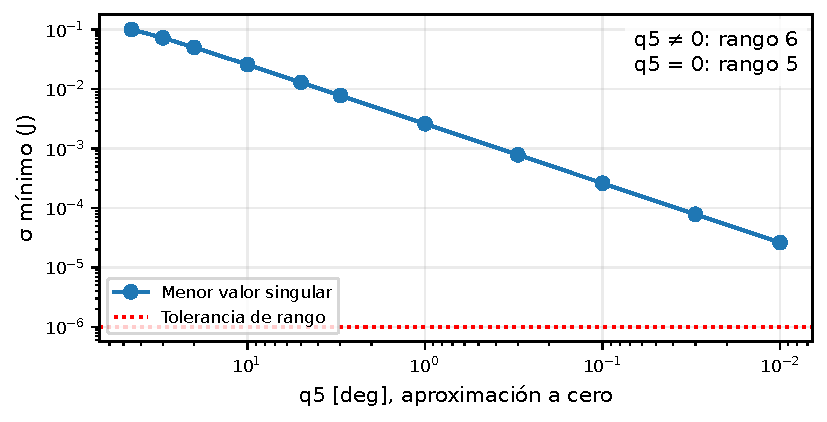
\includegraphics[width=\columnwidth]{D_singularidad_rango.pdf}
\caption{Al acercar $q_5$ a cero, el menor valor singular disminuye. En cero, el rango baja de 6 a 5.}\label{fig:sing}
\end{figure}
La Fig.~\ref{fig:sing} muestra esta aproximación. Para pedir ciertos movimientos de la herramienta cerca de esa postura, se necesitan velocidades articulares cada vez mayores. Eso no significa que el torque se vuelva infinito automáticamente: la singularidad describe una limitación de movimiento.

La postura inicial también tiene $q_5=0$. Podemos iniciar el LSPB desde ella porque planificamos directamente los ángulos de las articulaciones, sin exigir una velocidad de la herramienta en la dirección perdida.

\section{Torque con un modelo 1R}
Para estimar el esfuerzo del hombro usamos un modelo más sencillo de una sola articulación. Agrupamos los eslabones 2 a 6 y la pinza como si fueran un cuerpo rígido que gira sobre la articulación 2. Para obtener sus parámetros, mantenemos las demás articulaciones en la postura media del movimiento.

Los datos de masa e inercia provienen del modelo CAD usado en el código \cite{cad}. La masa agregada es 12,210 kg, la distancia del eje al centro de masa es 0,2491 m y la inercia equivalente es 1,2053 kg\,m$^2$. La pinza aporta 0,115 kg \cite{smc}; su posición se aproxima en el modelo.

El torque se calcula sumando el esfuerzo para acelerar y el esfuerzo para sostener el peso:
\begin{equation}
\tau=\underbrace{I_{eq}\ddot\theta}_{\text{inercia}}
+\underbrace{mg\ell_c\sin\theta}_{\text{gravedad}}.
\end{equation}
Usamos el mismo movimiento LSPB de la articulación 2. El ángulo $\theta=q_2-163{,}815^\circ$ se mide desde la vertical hacia abajo; este ajuste corresponde a la postura del cuerpo agrupado.

\begin{figure}[t]\centering
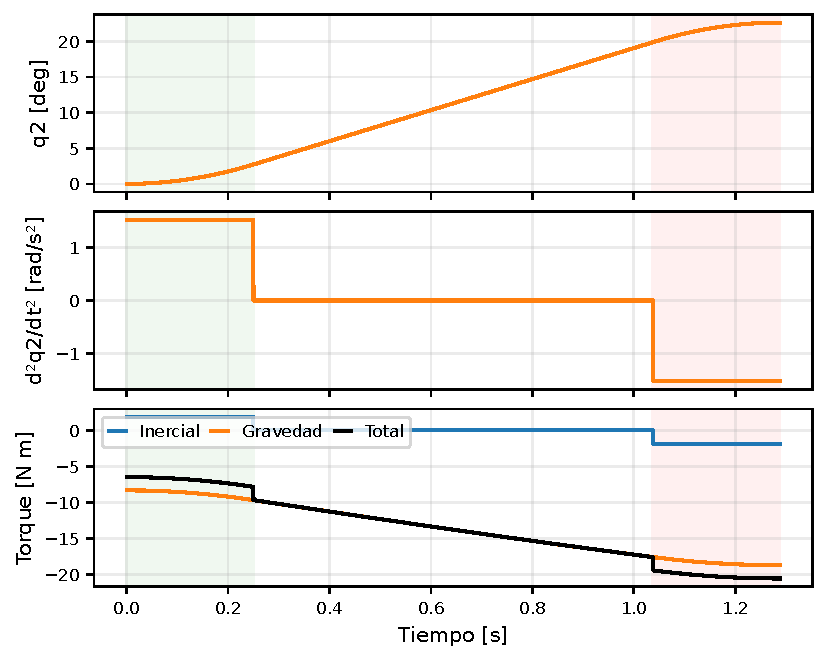
\includegraphics[width=\columnwidth]{E_torque_1R.pdf}
\caption{Movimiento del hombro y torque separado en inercia, gravedad y total.}\label{fig:torque}
\end{figure}
El mayor torque absoluto obtenido es 20,55 N\,m, justo antes de terminar el frenado. En ese momento se suman los efectos de gravedad y desaceleración. Después de detenerse, sin aceleración, queda el torque necesario para sostener el peso.

Durante el tramo de velocidad constante, el término de inercia es cero, pero el torque total no desaparece porque sigue actuando la gravedad. Ésta es la principal diferencia entre moverse a velocidad constante y no necesitar esfuerzo.

El modelo 1R se comparó con el modelo de seis articulaciones del código. El error RMS fue de 0,637 N\,m, equivalente al 4,5\% del RMS del torque del hombro. Es una comparación entre simulaciones que comparten datos; todavía no es una medición del brazo real.

\newpage
\section{Resultados y conclusiones}
El programa conectó la pose objetivo con los ángulos, la trayectoria, el Jacobiano y el torque. La ejecución aprobó las 32 verificaciones del cuaderno y las 49 pruebas del código.

En el ejemplo encontramos una sola solución dentro de los límites. El movimiento tarda 1,288 s y llega en reposo. La prueba de singularidad mostró que al alinear los ejes de la muñeca se pierde una dirección de movimiento. El modelo 1R permitió ver que el torque depende tanto de la aceleración como del peso del brazo.

Los resultados corresponden al ejemplo del cuaderno. Para otras poses asignadas por el docente se debe repetir el procedimiento. El modelo usa aproximaciones de masa, centro de masa y aceleración; no incluye fricción ni pruebas con el robot físico.

\begin{thebibliography}{4}
\bibitem{guia} IMT-342, ``Guía Oficial y Rúbrica de Evaluación: Hito 2,'' Universidad Católica Boliviana, repositorio docente \texttt{berquiroga/planificacion-UCB}, 2026.
\bibitem{abb} ABB Robotics, \emph{Product specification - IRB 120}, documento 3HAC035960-001, revisión W, 2023.
\bibitem{cad} L. N. Truc y N. T. Lam, ``Quasi-physical modeling of robot IRB 120 using Simscape Multibody for dynamic and control simulation,'' \emph{Turkish Journal of Electrical Engineering and Computer Sciences}, vol. 28, no. 4, pp. 1949--1964, 2020, doi: 10.3906/elk-1909-131.
\bibitem{smc} SMC Corporation, \emph{Parallel Type Air Gripper, Series MHZ2}, especificaciones del modelo MHZ2-16D(N).
\end{thebibliography}
\end{document}
